\chapter{Machine Learning and the Renormalization
  Group}\label{sec:comparison}
In the previous chapter, we considered two examples of ML in physical
investigations: neural networks used as a phase classifier and MCMC
sampler. Consider the superficial similarities between these neural
networks and our treatment of RG in \fref{sec:crit-phenomena}. The
classification example calls to mind the infinite RG limit in which
all disordered phases flow to one fixed point and all ordered phases
to another. Here, these fixed points would correspond to the values of
our label being either $0$ or $1$. The generative example is more
immediately similar, and the very language is analogous: we speak of
hidden layers that hierarchically decompose the input visible layer to
coarse-grained hidden layers. We might be tempted to ask: does a DBM
of, say, five layers learn to implement four iterations of some RG
procedure \sref{fig:rbm-rg}?

\begin{figure}[ht]
  \centering 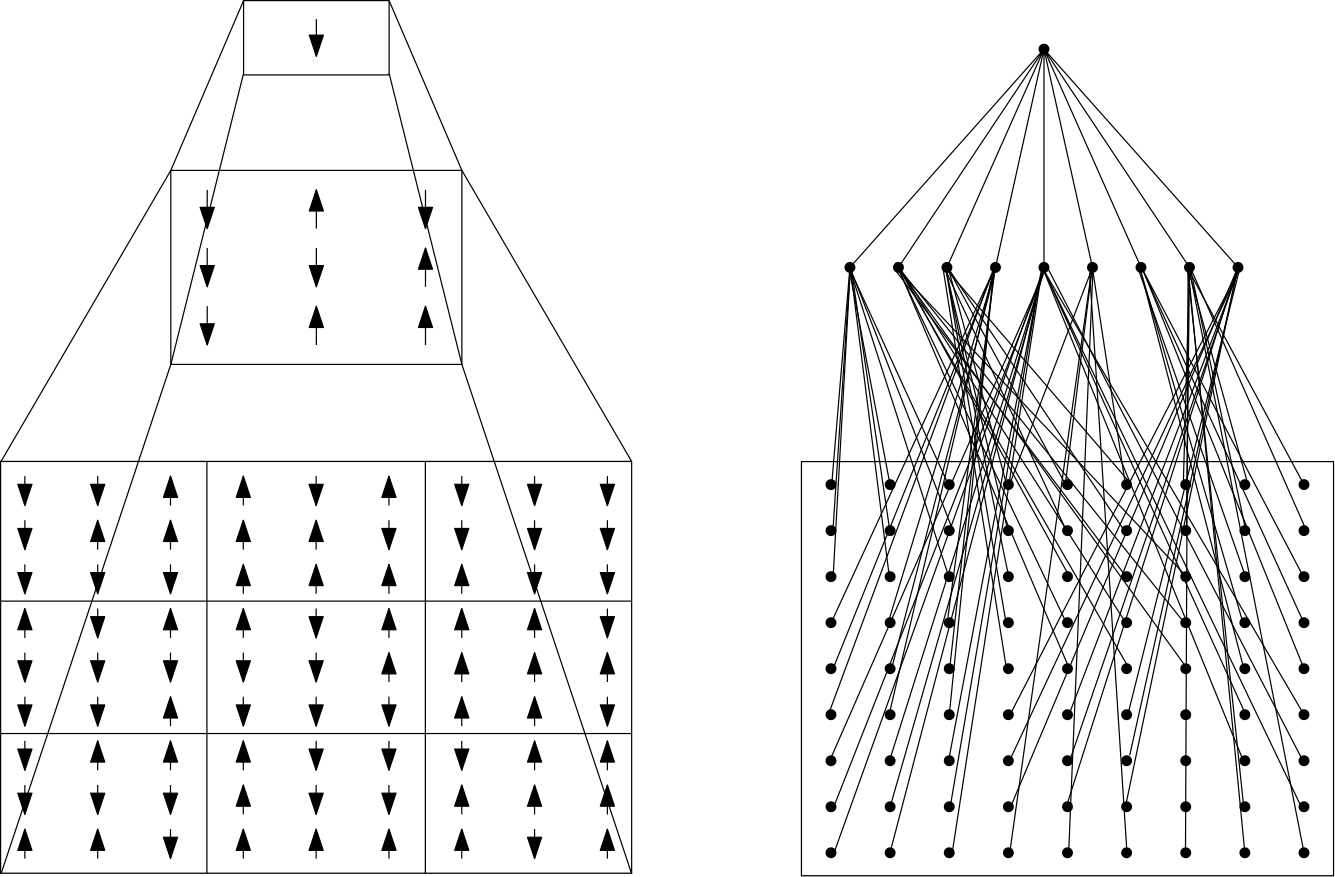
\includegraphics[width=0.5\textwidth]{figures/rg-rbm.png}
  \caption{Two iterations of block renormalization and a deep
    Boltzmann machine of three layers.\label{fig:rbm-rg} }
\end{figure}a


However, questions like this are too general. We have already seen two
examples of RBMs used for different goals, and what constituted relevant
information differed in either context. In RG, relevant information is
understood more narrowly: it is the long-distance information. If we
are to make comparisons between RG and RBMs, we must be more specific,
and this begins by being more precise in our definition of
``relevant'' information. Although Claude Shannon, the founder of
information theory, avoided this topic explicitly, Tishby et al.\
showed that information theory provides a natural and exact
formulation of relevant information: relevant information is simply
the information contained in one signal, $\bx$, about another
$\by$~\cite{tishby}. For our phase classifier, the relevant
information is the information contained in the Ising samples $\bx$
about the labels $\by$. Once we have trained RBMs for compression, the
relevant information is the information contained in the hidden layer
$\bh$ about the visible layer $\bv$. Information theory quantifies how
much information is shared between two signals with the mutual
information:
\begin{equation}%
  I(\bx; \by)\eqcolon\sum_{\bx,\by}P(\bx,\by)\log\left(\frac{P(\bx,\by)}{P(\bx)P(\by)}\right),\label{eq:mutual-info}
\end{equation}%
We see this quantity is minimized ($I(\bx;\by)=0$) when the random
variables are independent ($P(\bx,\by)=P(\bx)P(\by)$). It is maximized
when the variables are maximally dependent. We have a quantitatively
basis for extracting relevant information: maximizing mutual
information between appropriately chosen signals.

In the next chapter, we will derive the correct choice for $\bx$ and
$\by$ on lattice systems that recovers physically-relevant (i.e.\
long-distance) information. We then derive a variational proxy to the
mutual information that we can differentate and, thus, learn in a
neural network.

With the knowledge of an exact formulation of relevant information, we
can start investigating links between particular RG implementations
and RBMs. Such comparisons will revolve around the question of
relevance. What information does a given cost-function deem relevant?
Are there examples where this overlaps with our notions of physical
relevance? Let us consider a seminal example.

\section{A Comment on Mehta and Schwab's Equivalence}
As a first attempt, we will consider Mehta and Schwab's correspondence
between Kadanoff's variational procedure \pref{sec:kadanoff} with RBMs
trained by contrastive divergence
\pref{sec:rbm-generative-modeling}~\cite{mehta}. Specifically, we
consider the narrower case, of ``exact'' RG and ``exact'' RBMs. Exact
RG means that Kadanoff's transformation preserves \textit{all} the
information contained in the hidden system; i.e.\ the free energy of
the input and coarse-grained systems is exactly the same. Similarly,
an exact RBM has learnt to perfectly recreate its inputs
$P_{true}(\bx)=P_\theta(\bx)$ in \fref{eq:kld}; the RBM will have
reached a global minimum of the cost function.

First, Mehta and Schwab show that, under the above conditions, the two
transformations are equivalent under:%
\begin{equation}
  \bT_\theta(\bv, \bh)=-\bolds{E}_\theta(\bv,\bh)+\bolds{H}(\bv),
\end{equation}
and we provide the derivation in \fref{sec:mehta-equivalence}.

However, the exact case is not generally possible, and when it is, it
is often not particularly interesting. Exact RBM transformations
likely mean overfitting which is likely opposed to the aims of the ML
investigation. Exact RG transformations are few and far between, so
this correspondence would apply only under narrow circumstances. More
interesting then, would be to consider a non-exact comparison.

Here, the two approaches will vary: Kadanoff's variational method
operates at the level of free energies while contrastive divergence
works at the level of probabilities, and optimizations at these
different levels will not necessarily coincide. Still, there may still
be qualitative similarities. Pursuing this line of inquiry, Mehta and
Schwab train RBMs as described in
\fref{sec:rbm-generative-modeling}. They find that the RBMs learn to
couple hidden units to local blocks of visible units.\footnote{
  Crucially, this was not possible without \textit{regularization}, a
  technique that promotes sparse connections, between hidden and
  visible units see~\cite{mehta-review}.}
\begin{figure}[ht]
  \centering 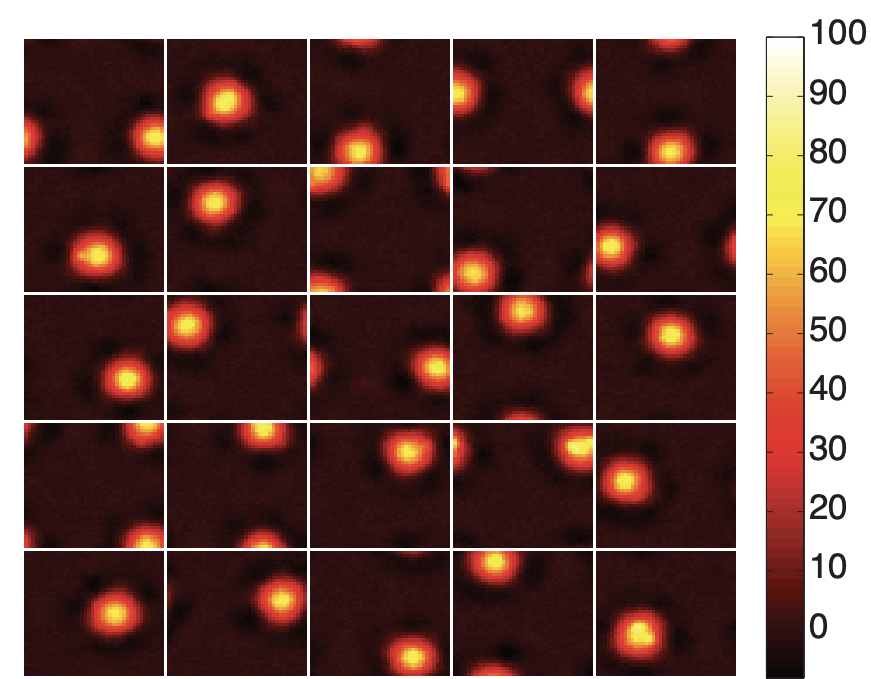
\includegraphics[width=0.5\textwidth]{figures/mehta.png}
  \caption{Visualization of the receptive filters of the hidden units
    in one of the layers of the DBM trained by Mehta and
    Schwab~\cite{mehta}. Each plot corresponds to one hidden unit, and
    each pixel corresponds to one spin in the initial layer. Higher
    intensities mean the hidden unit is more coupled to that
    spin. Indeed, we see that the RBM learns to couple local
    transformations. However, the transformations do not preserve
    nearest neighbor relations. This does not matter for the total
    amount of information stored in coarse-grained layers. In RG,
    these concerns do matter because they affect the practicality and
    interpretability of result~\cite{kjr}.\label{fig:fig:mehta} }
\end{figure}

Mehta and Schwab write:%
\begin{quote} Surprisingly, this local block spin structure emerges
  from the training process, suggesting the [deep neural network] is
  self-organizing to implement block spin
  renormalization~\cite{mehta}. % write out DNN somewhere.
\end{quote}

These RBMs may indeed learn a kind of block-spin
transformation. However, this block-spin transformation need not be
block-spin \textit{renormalization}. As Koch-Janusz and Ringel put it:
\begin{quote}
  [T]he usefulness (and practicality) of the RG procedure depends on
  choosing [the transformation] \ldots such that the effective
  Hamiltonian\ldots remains as short range as possible.~\cite{kjr}
\end{quote}
More precisely, in the Taylor expansion of our coarse-grain
Hamiltonians, the shortest range terms should dominate:
\begin{equation}%
  H(\bs)=-\sum_i K^{(1)}_{i} s_i - \sum_{\expect{i,j}}K^{(2)}_{ij}s_i s_j-\sum_{\expect{\expect{i,j}}}K^{(3)}_{ij}s_i s_j\ldots,
\end{equation}%
with $K^{(n)}$ are exponentially suppressed in $n$. In RG, we place
additional constraints on how to organize the information in
subsequent layers. Block renormalization procedures, including
Kadanoff's technique, respect the symmetries and topology of the
system under consideration. The locality of interactions means
neighboring visible blocks of spins become neighboring hidden
spins. Translational symmetry means the same transformation is applied
to each block.  Mehta and Schwab's RBMs will not, in general, satisfy
these two conditions.

Let us be more exact, rephrasing renormalization in probabilistic
terms: we parametrize our RG transformation as the conditional
probability distribution $P(\bh\rvert\bx)$, where $\bx$ is our initial
configuration and $\bh$ is the hidden or coarse-grained
configuration. Locality and translational invariance of the Ising
model mean we can factor the RG transformation into a product of local
single-block transformations. We divide the system into $M$ blocks,
$\bx\rightarrow\{v^{(1)}, v^{(2)},\ldots, v^{(M)}\}$, with
corresponding hidden units $\{h_1, h_2,\ldots,h_M\}$. Then we can
factor $P(\bh\rvert \bx)$ as:
\begin{equation}%
  P(\bh\rvert\bx)=\prod_{j=1}^M P(h_j\rvert \bv^{(j)}).\label{eq:prob-block-rg}
\end{equation}%
Consider what happens, when you permute the units in the hidden layer;
i.e., we use a different transformation $P(h_{j'}\rvert \bv^{(j)})$
where $j\neq j'$.  As long as our reverse rule, $P(\bx\rvert\bh)$ also
takes this into account, such a permutation has no impact on the
performance of Mehta and Schwab's contrastive divergence trained
RBMs. This is \textit{not} the case in RG\@. There is a unique
permutation of hidden layer degrees of freedom which maximizes the
above short range condition, and acceptable RG transformations
identify this permutation.

Furthermore, the block transformations that the RBM learns may not be
the same for each block. Compression and generation are invariant
under partial flips $h_j:(0,1)\rightarrow(1,0)$, for some fixed
$j$.\footnote{RG transformations are invariant under a collective flip
  of $\bh$.} Blocks of spins which were perfectly correlated in the
visible layer may be perfectly anticorrelated in the hidden
layer. Although the information content is the same, the hidden layer
Hamiltonian will take a more complicated form than is necessary, going
against notions of what is a good and practical RG procedure.

Mehta and Schwab fail to mention these conditions, so their suggestion
that RBMs learn block-spin renormalization falls short. However, if we
make these conditions explicit, we can easily recover a stronger
version of their claim. To do this, we introduce convolutional neural
networks (CNNs) as depicted in \fref{fig:cnn}. These are networks with
a special architecture: instead of all-to-all couplings, we explicitly
couple spins in the hidden layer to blocks in the visible
layer. Additionally, CNNs perform the same translation for each block
and respect the topology of the input system. Had they required a
convolutional architecture upfront, Mehta and Schwab may, indeed, have
successfully trained RBMs to learn even block renormalization.


\begin{figure}[]
  \centering 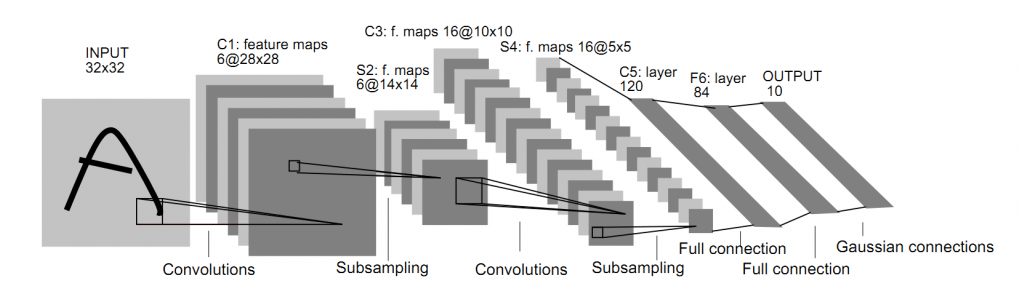
\includegraphics[width=\textwidth]{figures/cnn.png}
  \caption{This is LeNet-5, an example of a convolutional neural
    network used for digit recognition and a seminal
    architecture~\cite{lecun}.\label{fig:cnn} }
\end{figure}

From these observations, we can make the link between majority-rule
block-spin RG and ML fully precise.  In \fref{sec:majority-rule-rbm}, we
derive a equivalence between RBMs an RG, describing a parameterization
which implements the majority-rule:
$P(h_j|\bv^{(j)})=\sgn \sum_i v_i^{(j)}$.

\section{Relevant Information}
For the exact case discussed by Mehta and Schwab, we preserve the full
probability measure which necessarily preserves the long-distance
information. However, in the non-exact case, the KLD has no preference
for long-distance information over short-distance: all information is
valued equally. In the case of compression and generation, this is
acceptable: we have no a priori knowledge of which features in the
data are more important.

In RG, we have stronger requirements: transformations must favor
long-distance information over short-distance information. We can say
resolutely: RBMs trained with the KLD (even with the appropriate
convolutional architecture) need not learn acceptable RG
transformations. Perhaps in the case of the simple Ising model, the
KLD is an adequate heuristic. However, we have no guarantee that this
extends to novel systems. In fact, Koch-Janusz and Ringel showed that
RBMs trained with the KLD on the dimer model, another model from
statistical physics, couple to local fluctuations rather than to the
correct hidden variables~\cite{kjr}. We recall that appropriate
transformations for one system need not translate to others
\sref{sec:kadanoff}. Critique of Mehta and Schwab's paper revolves
primarily around the KLD being an inappropriate criterion for RG
transformations~\cite{lin, iso}.

In reply, Mehta and Schwab point out that Kadanoff's method also
offers no guarantee of extracting the correct physical information. We
come back to the difficulty of devising appropriate RG techniques, and
the need for creativity. In fact, this need for intuition in RG is
mirrored quite clearly in ML\@. Decisions regarding model
architectures and cost functions require creativity on the part of the
researcher. Both fields would benefit from a clearer understanding of
when techniques will and will not work. In the next chapter, we will
see that information theory may provide the framework to answer
questions like these, and we will encounter a system-independent
formulation of RG\@. This might mean better, more efficient models in
both disciplines.
